%!TEX root = ../main.tex


\section{Van Benthem's Theorem}\label{sec:van-benthem-theorem}
Van Benthem's theorem shows that modal logic corresponds to the bisimulation-invariant subset of first order logic~\cite{van1983modal}, which holds even in finite structures~\cite{Rosen97}.
We can prove an analogous theorem for the forward guarded fragment, using our modified notion of bisimulation:

\begin{theorem}
  The following two statements are equivalent:
  \begin{enumerate}
    \item $\phi(\bar{x}) \in \Logic{FO}$ is invariant under \FGF-bisimulation in finite models
    \item $\phi(\bar{x})$ is logically equivalent to a \FGF~formula in finite models
  \end{enumerate}
\end{theorem}

The prove this theorem, we use the following oberservation by Otto~\cite{Otto04}:
\begin{observation}
  Let $\bisimto$ have finite approximations $\bisimto^{\ell}, \ell \in \mathbb{N}$.
  Assume that each $\bisimto^{\ell}$ has finite index for every finite relational vocabulary.
  Let $\Logic{L} = \bigcup_{\ell}{\Logic{L}^{\ell}}$ be a logic, each stratum $\Logic{L}^{\ell}$ closed under disjunctions.
  Assume that each $\Logic{L}^{\ell}$ is invariant under $\bisimto^{\ell}$ and that each $\bisimto^{\ell}$-class is definable by a formula of $\Logic{L}^{\ell}$.

  Then the following are equivalent, both in the sense of classical model theory and of finite model theory:
  \begin{enumerate}[(i)]
    \item Every FO formula that is $\bisimto$-invariant is invariant under $\bisimto^{\ell}$ for some $\ell$.
    \item Every FO formula that is $\bisimto$-invariant is equivalent to some formula in $\Logic{L}$.
  \end{enumerate}
\end{observation}

We have shown previously that $\FGF$, $\bisimto_{\FGF}$ and $\bisimto_{\FGF}^{\ell}$ satisfy the preconditions of this observation.
Hence it is sufficient to show condition (i).
Following Otto, we prove this condition by upgrading \FGF~bisimulation to a stronger form of bisimulation: \GF~bisimulation:

\begin{proof}
  Let $\phi$ be an $\FO$ formula invariant under $\bisimto_{\FGF}$.
  $\phi$ is then also invariant under $\bisimto_{\GF}$, since $\bisimto_{\GF}$ is stronger than $\bisimto_{\FGF}$.
  This implies that there exists a finite $g$ such that $\phi$ is invariant under $\bisimto_{\GF}^{g}$, as a result of Otto's proof of the van Benthem theorem for \GF~\cite{Otto2012}.

  By theorem \todo[inline,inlinewidth=5cm,noinlinepar]{TODO: upgrading theorem}, there is a finite $\ell$ and $\theta$ for this $g$ such that for arbitrary models, $~^{\ell}$-\FGF-bisimilarity implies that their $\theta$-unravelings are $g$-\GF-bisimilar.
  Let $\str{A}, \bar{a} \bisimto_{\FGF}^{\ell} \str{B}, \bar{b}$ be two $\ell$-\FGF-bisimilar models.
  Then, $\str{A}, \bar{a} \models \phi(\bar{x}) \implies \str{B}, \bar{b} \models \phi(\bar{x})$ (and vice-versa by symmetry), as can be seen following \cref{fig:fgf-to-gf-upgrade}:
  \begin{itemize}
    \item $\phi(\bar{x})$ is preserved in $\str{A}^{\rightarrow}_{\theta}, \overrightarrow{a}$, since $\phi(\bar{x})$ is preserved under \FGF-bisimulation by assumption and the unraveling is fully \FGF-bisimlar
    \item $\phi(\bar{x})$ is preserved in $\str{B}^{\rightarrow}_{\theta}, \overrightarrow{b}$ since the unravelings are $\bisimto_{\GF}^{g}$ equivalent and $\phi$ is invariant under $\bisimto_{\GF}^{g}$
    \item $\phi(\bar{x})$ is preserved in $\str{B}, \bar{b}$ again since the unravelings are \FGF-bisimilar
  \end{itemize}
  This shows that $\phi$ is invariant under $\bisimto_{\FGF}^{\ell}$, completing the proof.
\end{proof}

\begin{figure}
  \centering
  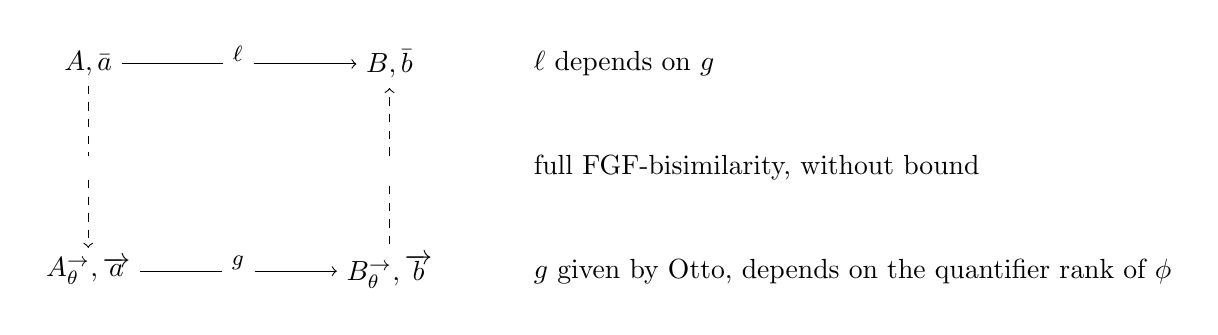
\begin{tikzpicture}
    \matrix[row sep=2em, column sep=3em]
    {
        \node (a) {$\str{A}, \bar{a}$}; &
        \node[font=\large] (sim_ab) {$\bisimto_{\FGF}^{\ell}$}; &
        \node (b) {$\str{B}, \bar{b}$}; &
        \node[anchor=west] {$\ell$ depends on $g$}; \\

        \node[font=\large] (sim_a_unravel) {$\bisimto_{\FGF}$}; &
        \node {}; &
        \node[font=\large] (sim_b_unravel) {$\bisimto_{\FGF}$}; &
        \node[anchor=west] {full FGF-bisimilarity, without bound}; \\

        \node (a_unravel) {$\str{A}^{\rightarrow}_{\theta}, \overrightarrow{a}$}; &
        \node[font=\large] (sim_unravel) {$\bisimto_{\GF}^{g}$}; &
        \node (b_unravel) {$\str{B}^{\rightarrow}_{\theta}, \overrightarrow{b}$}; &
        \node[anchor=west] {$g$ given by Otto, depends on the quantifier rank of $\phi$}; \\
    };

    \draw[->] (a) -- (sim_ab) -> (b);
    \draw[dashed,->] (a) -- (sim_a_unravel) -> (a_unravel);
    \draw[->] (a_unravel) -- (sim_unravel) -> (b_unravel);
    \draw[dashed,->] (b_unravel) -- (sim_b_unravel) -> (b);
  \end{tikzpicture}
  \caption{Upgrading FGF to GF bisimulation}
  \label{fig:fgf-to-gf-upgrade}
\end{figure}
